%--------------------------------------------------------------------------------------------------------------
\begin{Exercise}
A student named Ralph has used a voltage divider to build a 2-volt DC voltage supply, shown below on the left.  It turns out there is a very useful theorem by a fellow named Thevenin, which says roughly the following:
\begin{quote}
``Any collection of voltage sources and resistors (even the crazy middle figure below!) is functionally equivalent to a single voltage source $V_{\rm Th}$ and a single internal resistance $R_{\rm Th}$ as shown on the right.  No measurement at $V_{\rm out}$ can distinguish between the two circuits.''  ---L\'eon Charles Th\'evenin (heavily paraphrased).
\end{quote}
In this problem, you will calculate the values of $V_{\rm Th}$ and $R_{\rm Th}$ for the equivalent circuit of Ralph's voltage supply. 

\begin{center}
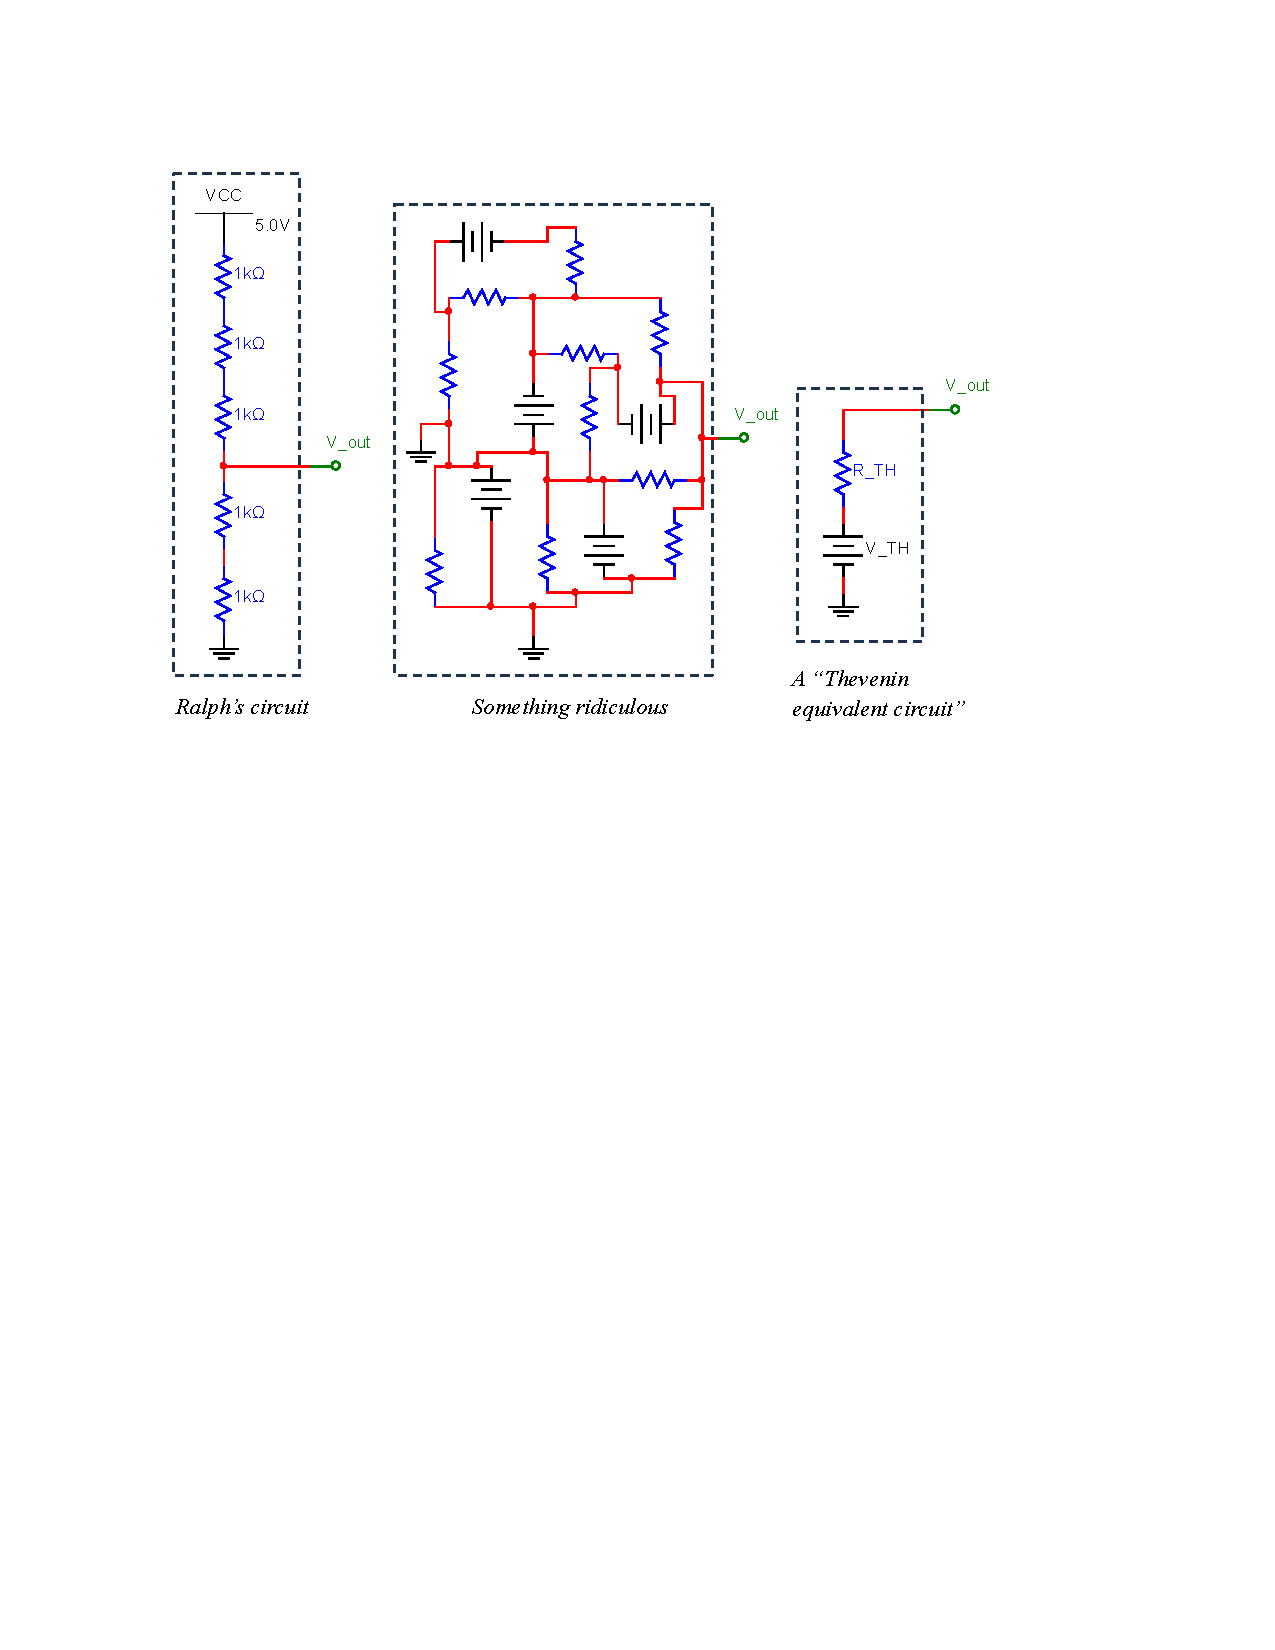
\includegraphics[scale=0.9]{M_problems/the_basics/thevenin_equivalence.pdf}
\index{color page}
\end{center}

(a)~What is the open-circuit voltage of the Thevenin equivalent circuit on the right, in terms of $V_{\rm Th}$ and $R_{\rm Th}$?  (Yes, this is easy.)  
(b)~What is the short-circuit current of the Thevenin equivalent circuit on the right?  (Also easy.)
(c)~What is the open-circuit voltage of Ralph's circuit?  
(d)~What is the short-circuit current of Ralph's circuit?  
(e)~From your previous parts what are the values of $V_{\rm Th}$ and $R_{\rm Th}$ for Ralph's circuit?  
(f)~Ralph does the same calculation that you did, and says, ``Hey, it looks like the output impedance of my circuit is 1.2~k$\Omega$.''  Is \textit{output impedance} the right thing for Ralph to call it?
\end{Exercise}
\begin{Answer}
(a) It's just $V_{\rm Th}$ (b) $V_{\rm Th}$ and $R_{\rm Th}$ (c) 2 V (d) 1.67 mA (e) 2 V and 1.2 k$\Omega$ (f)~Sure, that's basically what it is.  In this context, ``output impedance/resistance'' or ``internal resistance'' or ``Thevenin equivalent resistance'' basically all mean the same thing.
\end{Answer}


%--------------------------------------------------------------------------------------------------------------
\begin{Exercise}
In this problem, you will test whether Ralph's circuit in the previous problem is equivalent to a Thevenin equivalent circuit with $V_{\rm Th}=2$~volts and $R_{\rm Th}=1.2\kohm$, by checking the behavior of a circuit with a single, arbitrarily chosen load resistor $R_{\rm L}$. Suppose a load  $R_{\rm L}=2.7\kohm$ is connected between Ralph's output and ground.  (a)~Calculate the voltage across and current through $R_{\rm L}$ by analyzing the circuit in the diagram below on the left.  (b)~Calculate the voltage and current for $R_{\rm L}$ by analyzing the circuit in the diagram below on the right.  (c)~Are they the same?  (d)~Does this count as a ``proof'' of Thevenin's theorem?
\begin{center}
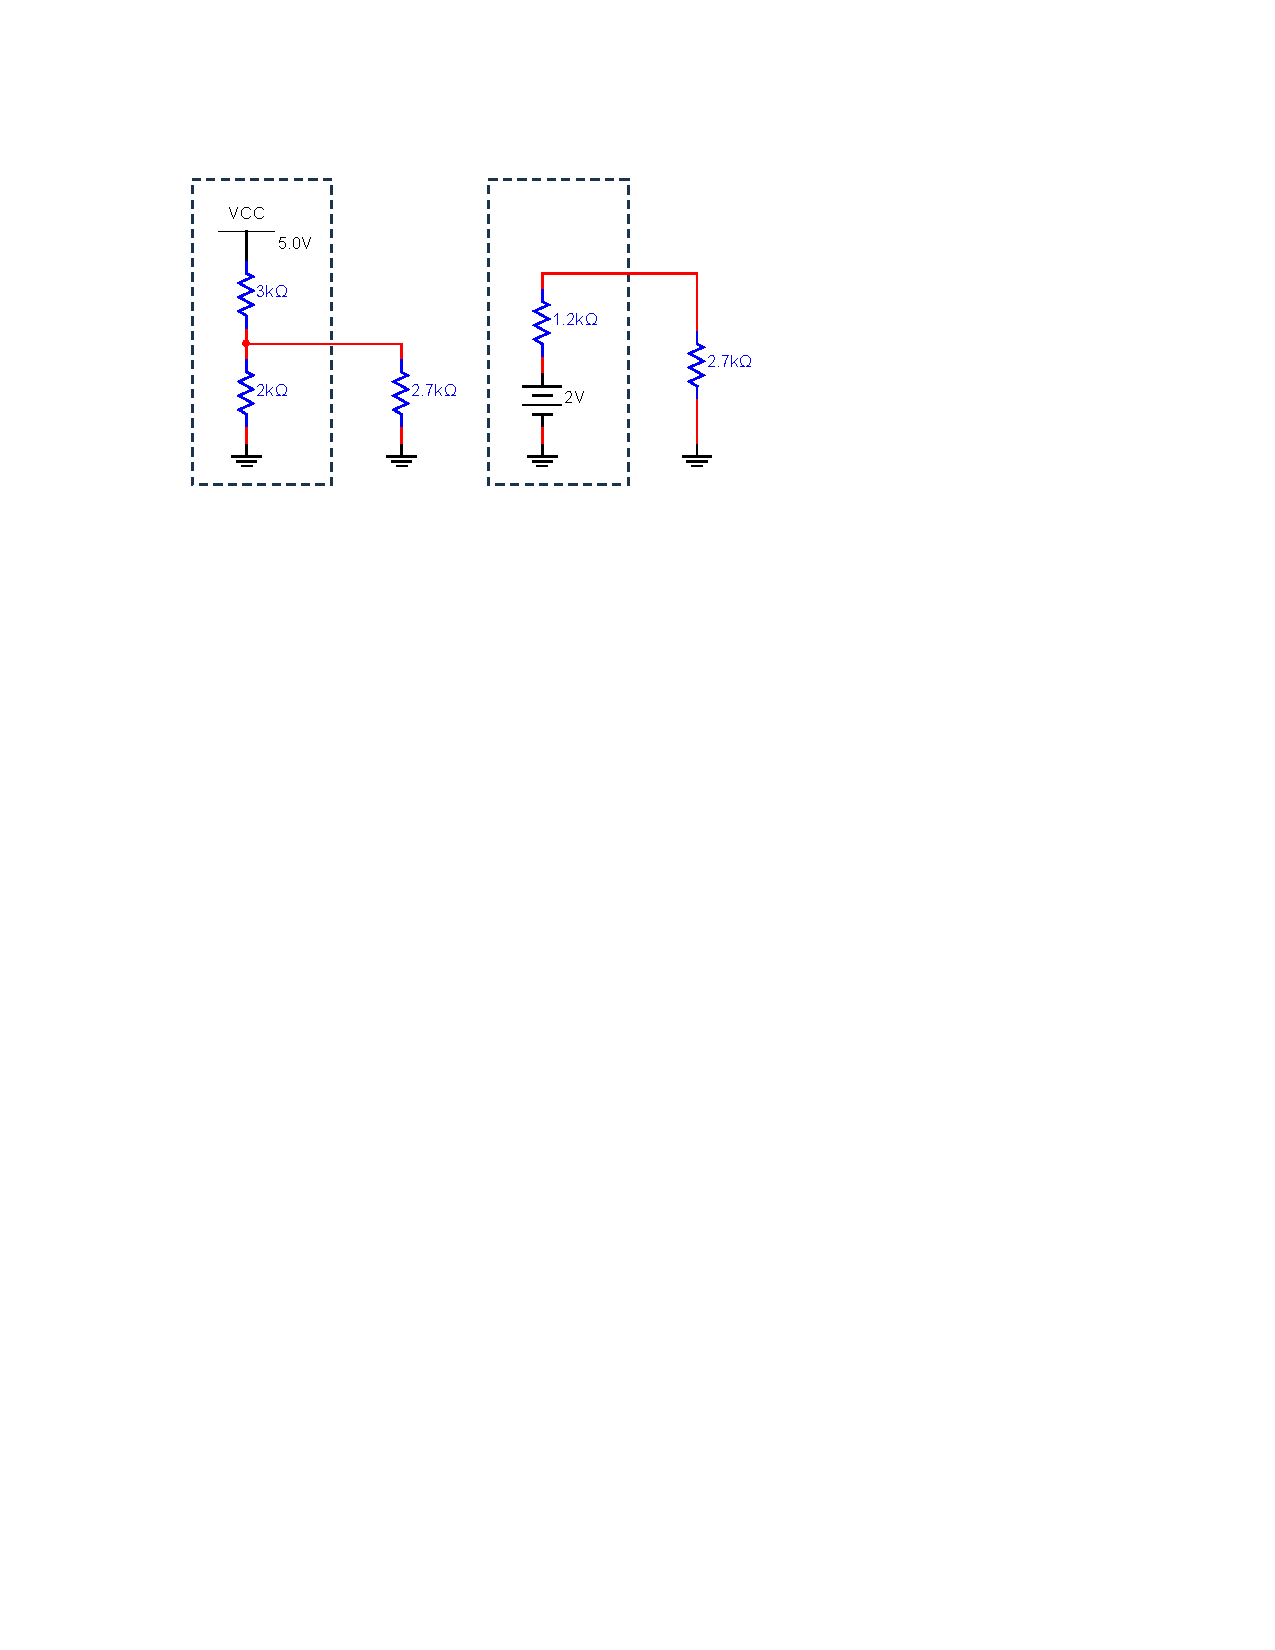
\includegraphics[scale=0.9]{M_problems/the_basics/thevenin_equivalence2.pdf}
\index{color page}
\end{center}
\end{Exercise}
\begin{Answer}
(a)~1.38~V and 513~$\mu$A  (c)~They'd better both be the same! (d)~No, it's not a general proof, because you demonstrated it only for one specific load (a single $2.7\kohm$ resistor) connected to one specific circuit made by some fake guy named Ralph.  But if you see this kind of thing enough times, it does start to seem convincing.  :-)
\end{Answer}

